%--------------------------------------------------------------------%
% Page          : Chapter 2 - Kajian Pustaka (Literature Review)
%--------------------------------------------------------------------%

\chapter{KAJIAN PUSTAKA}
\label{sec:kajian-pustaka}

Pada bab ini dijelaskan mengenai pustaka yang digunakan sebagai landasan ilmiah penelitian dan pustaka penelitian yang telah dilakukan sebelumnya terkait penelitian yang akan dilakukan.

\section{Cloud Computing}
\label{sec:cloud-computing}

\begin{figure}[htbp]
    \centering
    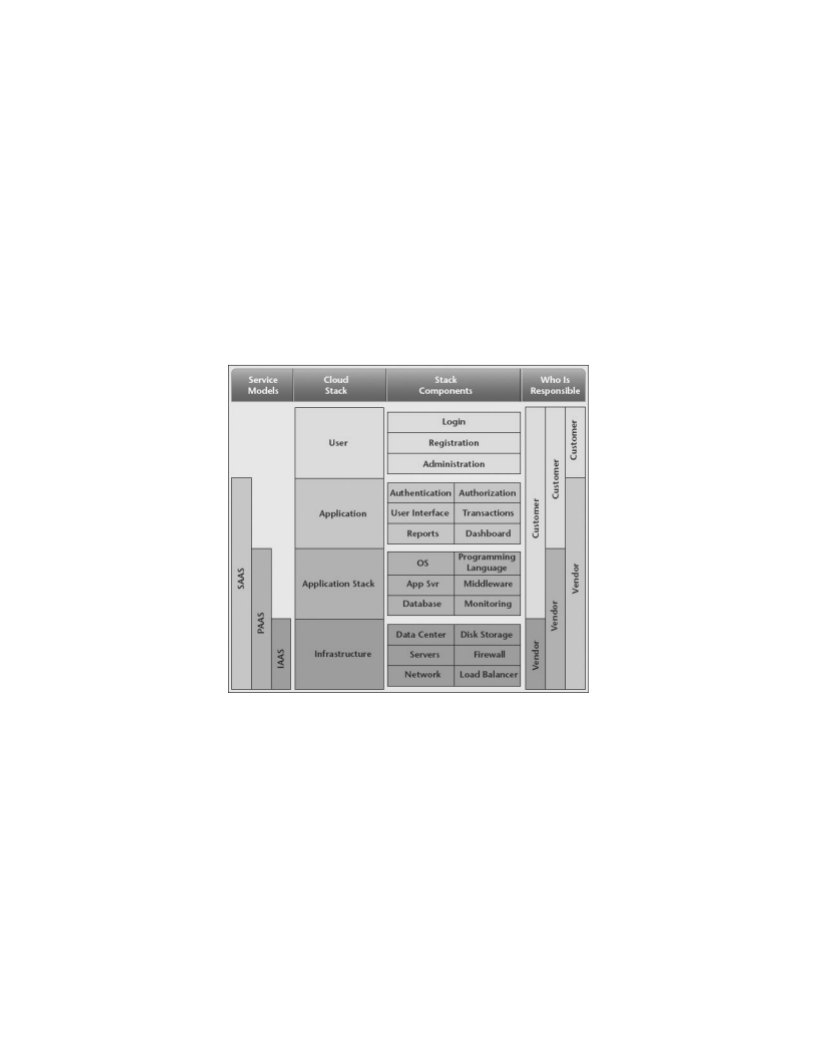
\includegraphics[keepaspectratio, width=0.7\textwidth]{src/resources/figures/image3.png}
    \caption{Cloud services and division of responsibilities \citep{kavis2014}}
    \label{fig:cloud-services}
\end{figure}

Cloud computing, menurut National Institute of Standards and Technology (NIST), adalah model yang menyediakan akses \emph{on-demand} ke kumpulan jaringan komputasi yang dapat dikonfigurasi. Model ini mencakup tiga layanan utama: \emph{Infrastructure-as-a-Service} (IaaS) yang menawarkan sumber daya virtual yang dapat diskalakan; \emph{Platform-as-a-Service} (PaaS) yang menyediakan alat dan middleware untuk pengembang; dan \emph{Software-as-a-Service} (SaaS) yang menyediakan aplikasi perangkat lunak melalui internet \citep{mell2011nist}. Peralihan dari komputasi tradisional ke model berbasis layanan ini didorong oleh kemajuan dalam virtualisasi, penyimpanan, dan daya pemrosesan \citep{malathi2011cloud}.

Teknologi kontainer, yang didukung oleh platform seperti Docker, memudahkan pengelolaan kontainer dan membuka jalan bagi alat orkestrasi seperti Kubernetes \citep{yadav2019docker}. Kubernetes telah merevolusi orkestrasi kontainer dengan mengotomatiskan penerapan, penskalaan, dan manajemen aplikasi yang terkontainerisasi \citep{pahl2019cloud}. Selain itu, model komputasi tanpa server seperti \emph{Function as a Service} (FaaS) lebih lanjut menyederhanakan manajemen infrastruktur, memungkinkan pengembang fokus pada penulisan kode \citep{wurster2018modeling}.

\subsection{Container \& Kubernetes}
\label{sec:container-kubernetes}

Kontainer telah menjadi teknologi utama dalam komputasi awan, menawarkan alternatif yang lebih efisien dibandingkan mesin virtual tradisional (VM). Berbeda dengan VM yang memerlukan sistem operasi lengkap, kontainer berbagi kernel dengan sistem host dan mengisolasi lingkungan eksekusi aplikasi, mengurangi overhead dan meningkatkan kinerja. Isolasi ini dicapai melalui \emph{namespace} dan \emph{control group}---fitur Linux yang dapat membatasi akses dan penggunaan sebuah proses, memungkinkan \emph{multi-tenancy} yang aman dan kontrol alokasi sumber daya. Docker, menyediakan platform yang menyederhanakan manajemen \emph{package}, distribusi, dan manajemen aplikasi yang terkontainerisasi.

\begin{figure}[htbp]
    \centering
    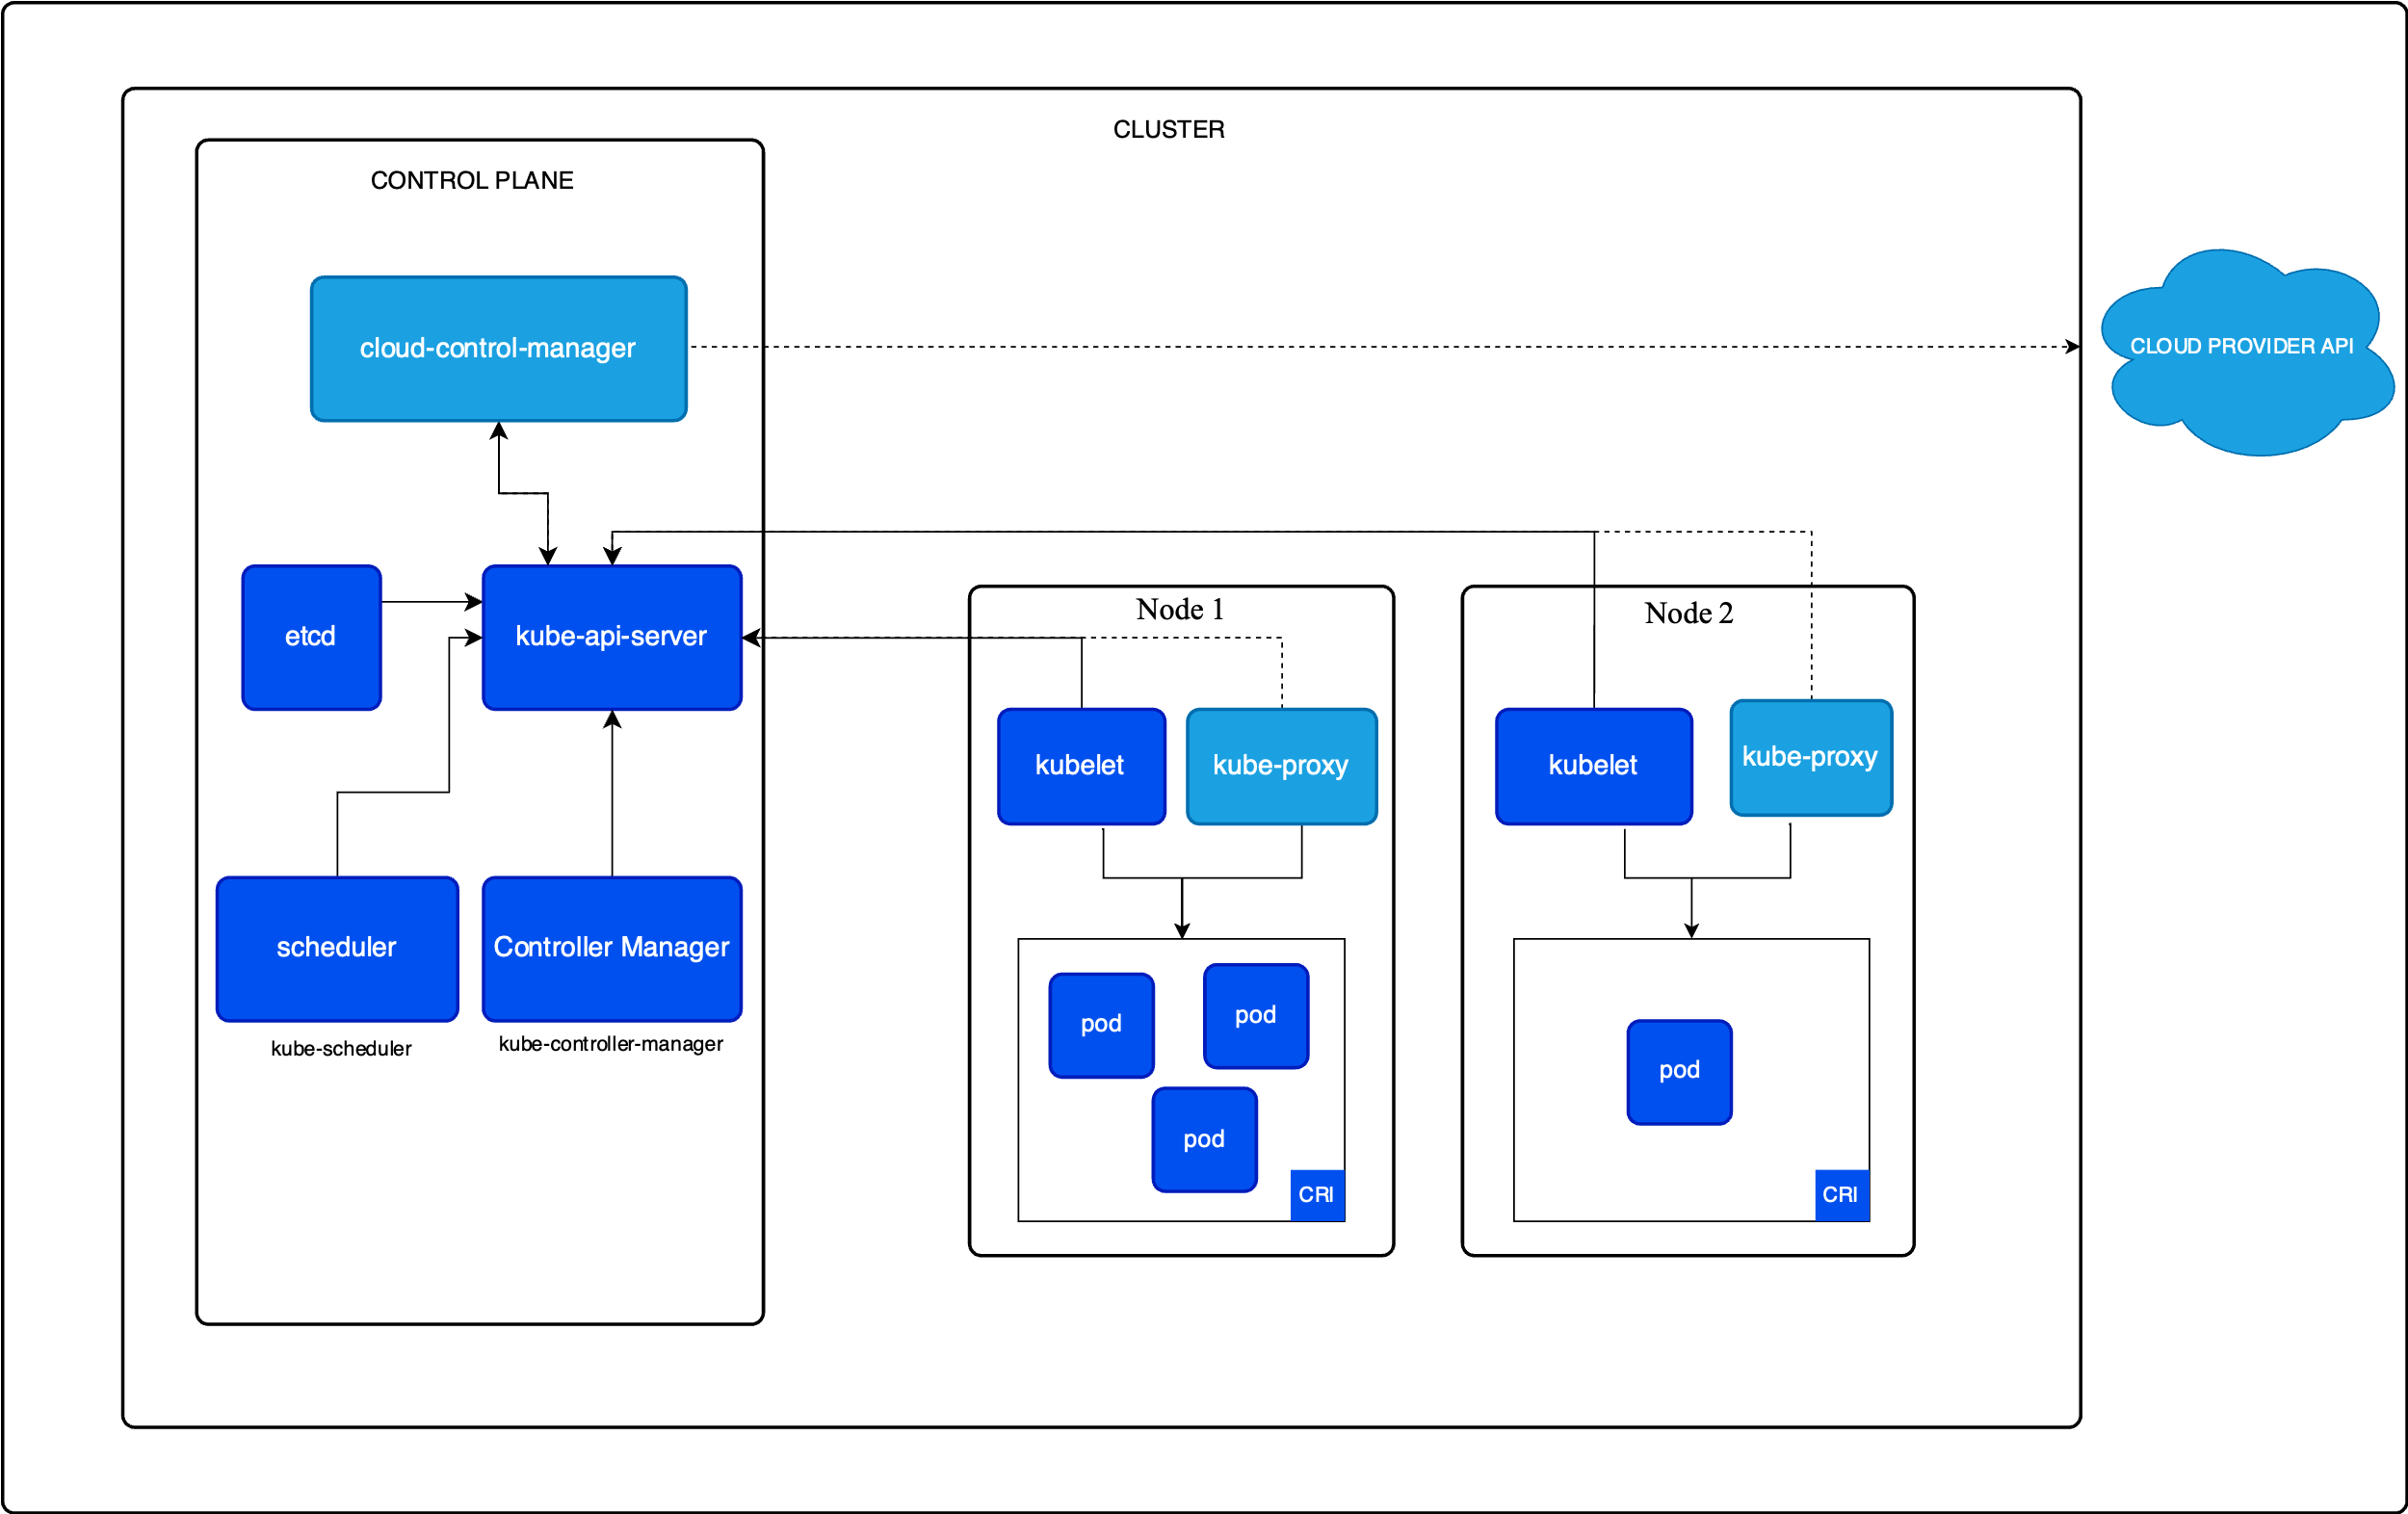
\includegraphics[keepaspectratio, width=0.8\textwidth]{src/resources/figures/image6.png}
    \caption{Architecture of a Kubernetes cluster}
    \label{fig:kubernetes-architecture}
\end{figure}

Seiring dengan meluasnya penggunaan kontainer, kebutuhan akan orkestrasi mereka memunculkan Kubernetes. Kubernetes adalah platform open-source yang dirancang untuk mengotomatisasi penerapan, penskalaan, dan operasi kontainer aplikasi. Platform ini mengelompokkan kontainer yang membentuk aplikasi ke dalam unit logis untuk memudahkan manajemen dan penemuan. Kubernetes menyediakan kerangka kerja untuk menjalankan sistem terdistribusi secara andal, dengan penemuan layanan dan penyeimbangan beban, orkestrasi penyimpanan, pengguliran otomatis dan pembatalan pengguliran, serta kemampuan penyembuhan diri.

Komponen utama dari \emph{control plane} meliputi:

\begin{itemize}
    \item \textbf{etcd}: Penyimpanan key-value yang persisten, ringan, dan terdistribusi, menyimpan data konfigurasi, status, dan metadata kluster.
    \item \textbf{kube-api-server}: Server API yang berfungsi sebagai antarmuka depan untuk \emph{control plane}.
    \item \textbf{kube-scheduler}: Komponen yang memantau pod baru yang belum memiliki node dan memilih node berdasarkan kriteria penjadwalan.
    \item \textbf{kube-controller-manager}: Menjalankan proses kontrol yang mengatur status kluster.
    \item \textbf{cloud-control-manager}: Menghubungkan kluster dengan API penyedia cloud.
\end{itemize}

Pada tingkat node, komponen utama meliputi:

\begin{itemize}
    \item \textbf{kubelet}: Agen yang berjalan di setiap node yang memastikan kontainer berjalan dalam pod.
    \item \textbf{kube-proxy}: Proxy jaringan yang menjaga aturan jaringan untuk komunikasi pod.
    \item \textbf{Container Runtime Interface (CRI)}: Antarmuka untuk runtime kontainer agar terintegrasi dengan kubelet.
    \item \textbf{Pod}: Unit terkecil yang dapat dibuat dan dikelola di Kubernetes.
\end{itemize}

\subsection{Function as a Service and Serverless}
\label{sec:faas-serverless}

\begin{figure}[htbp]
    \centering
    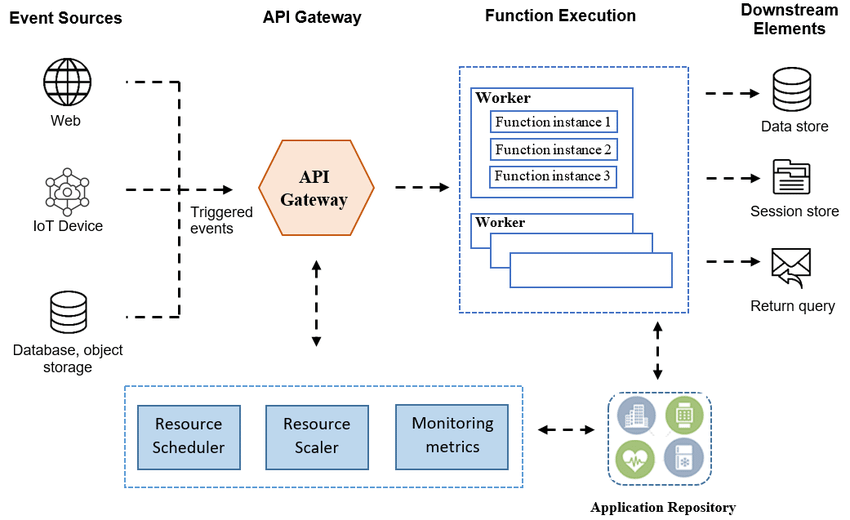
\includegraphics[keepaspectratio, width=0.6\textwidth]{src/resources/figures/image8.png}
    \caption{Serverless Architecture \citep{mampage2022holistic}}
    \label{fig:serverless-architecture}
\end{figure}

\emph{Function as a Service} (FaaS) atau serverless, merupakan model layanan cloud yang memungkinkan pengembang untuk menerapkan fungsi individu---blok kode yang dipicu oleh peristiwa tertentu. FaaS menyembunyikan infrastruktur dasar, termasuk server, sistem operasi, dan bahkan lingkungan eksekusi aplikasi, sehingga pengembang dapat fokus hanya pada penulisan logika bisnis.

Dalam arsitektur serverless, penyedia cloud bertanggung jawab untuk menjalankan fungsi sebagai respons terhadap peristiwa dan sepenuhnya mengelola infrastruktur yang mendasarinya. Pelanggan dikenakan biaya berdasarkan jumlah sumber daya yang benar-benar digunakan oleh aplikasi mereka, bukan berdasarkan unit kapasitas yang telah dibeli sebelumnya. Model ini dapat menghasilkan penghematan biaya yang signifikan karena menghilangkan kebutuhan untuk menjalankan kapasitas server yang tidak digunakan secara terus-menerus, namun akan menjadi mahal apabila terdapat beban konstan yang memerlukan sumber daya secara terus menerus.

\section{Integrasi Antara Kluster Kubernetes dan Serverless}
\label{sec:integrasi-kubernetes-serverless}

Seiring dengan pertumbuhan komputasi serverless, interaksi antara \emph{Function as a Service} (FaaS) dan Kubernetes menjadi semakin relevan. Sementara Kubernetes mengorkestrasi kontainer dengan efisien, komputasi serverless dapat menangani lonjakan peristiwa dengan cepat tanpa perlu mengelola server secara langsung. Mengintegrasikan keunggulan Kubernetes dan FaaS memungkinkan mekanisme distribusi lalu lintas yang secara dinamis dapat menyesuaikan skala dengan permintaan beban kerja, sambil mengoptimalkan biaya dan kinerja.

Strategi integrasi melibatkan konfigurasi \emph{deployment} di mana Kubernetes mengelola layanan jangka panjang yang konstan dan predictable, sementara fungsi serverless menangani tugas-tugas singkat ketika layanan kubernetes belum melakukan scalling sehingga tidak dapat dilayani. Model hibrida ini berpotensi menawarkan yang terbaik dari kedua dunia: kapabilitas orkestrasi dan manajemen Kubernetes serta model on-demand dan pay-as-you-go dari serverless.

\section{Cloud Application Performance}
\label{sec:cloud-performance}

Menentukan seberapa layanan cloud memenuhi ekspektasi pengguna dan \emph{Service Level Agreements} (SLA). Untuk memastikan bahwa aplikasi cloud beroperasi secara optimal, beberapa metrik kunci digunakan untuk mengevaluasi berbagai aspek kinerja.

\subsection{SLA Violation}

Pelanggaran SLA adalah salah satu indikator utama dalam penilaian kinerja aplikasi cloud. Pelanggaran ini terjadi ketika layanan gagal memenuhi ketentuan yang disepakati dalam SLA. Untuk mengukur pelanggaran SLA, dua metrik utama yang digunakan adalah tingkat keberhasilan dan jumlah tugas yang gagal \citep{aslanpour2020performance}.

\subsection{Request Response Time}

Waktu respons permintaan mencerminkan seberapa cepat aplikasi cloud dapat merespons permintaan pengguna. Metrik ini mencakup beberapa aspek, yaitu waktu berjalan, keterlambatan, dan \emph{tail latency}. \textbf{Waktu berjalan} mengukur durasi total untuk menyelesaikan suatu tugas. \textbf{Keterlambatan} diukur sebagai selisih antara waktu penyelesaian aktual dan yang diharapkan. \emph{\textbf{Tail latency}}, yang merupakan waktu respons di persentil tertinggi, memberikan gambaran tentang performa dalam kondisi beban puncak.

\subsection{Resource Utilization}

Resource Utilization mencakup alokasi, utilisasi, dan biaya. Alokasi sumber daya mengacu pada penugasan CPU, memori, dan bandwidth yang optimal. Utilisasi sumber daya diukur sebagai persentase dari kapasitas total yang digunakan. Biaya terkait dengan penggunaan sumber daya dihitung berdasarkan model pay-as-you-go.

\section{Algorithm and Prediction Model}
\label{sec:algorithm-prediction}

Dalam konteks manajemen lalu lintas dan penskalaan dinamis pada layanan cloud containerized, algoritma dan model prediksi memainkan peran penting dalam memprediksi beban kerja dan mengoptimalkan alokasi sumber daya.

\subsection{LSTM}

LSTM adalah pengembangan dari \emph{recurrent neural network} (RNN) yang dirancang untuk dapat belajar dan mengingat hubungan serta pola antara data yang berurutan dalam jangka panjang. Design dari LSTM memungkinkan untuk mengatasi permasalahan \emph{vanishing gradient} pada jaringan RNN. Satu sel LSTM terdiri dari gerbang input, output, dan forget yang berfungsi mengontrol aliran data.

\subsection{GRU}

\emph{Gated Recurrent Unit} (GRU) adalah varian dari RNN yang lebih sederhana dibandingkan LSTM, dengan mekanisme kontrol yang lebih sedikit. Terdiri dari hanya dua gerbang, sehingga lebih cepat dalam proses \emph{training} dan \emph{inference}, dengan tetap mempertahankan kemampuan untuk menangani ketergantungan jangka panjang \citep{mondal2023toward}. \emph{Update gate} menggabungkan fungsi dari \emph{input} dan \emph{forget} gate pada LSTM, bertanggung jawab mengatur informasi baru dan yang akan disimpan dalam sel. \emph{Reset gate} mengatur bagaimana informasi baru diintegrasikan dengan data sebelumnya.

\section{Kubernetes Scalling Strategy}
\label{sec:kubernetes-scaling}

Strategi \emph{scaling} pada aplikasi berfungsi agar aplikasi dapat menangani beban kerja yang berubah-ubah secara efisien. Kubernetes mendukung strategi \emph{scalling} secara horizontal, yang menambah jumlah \emph{deployment}, dan \emph{scalling} secara vertikal, yang menyesuaikan alokasi sumber daya dari pod yang ada.

\subsection{Kluster \& Pod Autoscaller}

\begin{enumerate}
    \item \textbf{Cluster Autoscaler}
\end{enumerate}

Cluster Autoscaler adalah mekanisme yang menyesuaikan jumlah node dalam kluster Kubernetes berdasarkan kebutuhan sumber daya pod. Jika pod baru tidak dapat dijadwalkan karena kekurangan sumber daya, Cluster Autoscaler akan menambahkan node baru. Sistem ini memerlukan waktu 2-5 menit dalam melakukan perubahan terhadap alokasi sumber daya.

\begin{enumerate}
    \setcounter{enumi}{1}
    \item \textbf{Pod Autoscaler}
\end{enumerate}

\textbf{Horizontal Pod Autoscaler (HPA)} secara otomatis akan menambah atau mengurangi jumlah replika pod berdasarkan metrik seperti CPU dan penggunaan memori. \emph{Scalling} cenderung lebih responsif terhadap perubahan beban kerja, dapat berubah kurang dari 30 detik.

\textbf{Vertical Pod Autoscaler (VPA)} menyesuaikan alokasi sumber daya (CPU dan memori) dari pod yang ada berdasarkan kebutuhan beban kerja.

\subsection{Metode ElaX dalam Scalling Kluster}
\label{sec:metode-elax}

\begin{figure}[htbp]
    \centering
    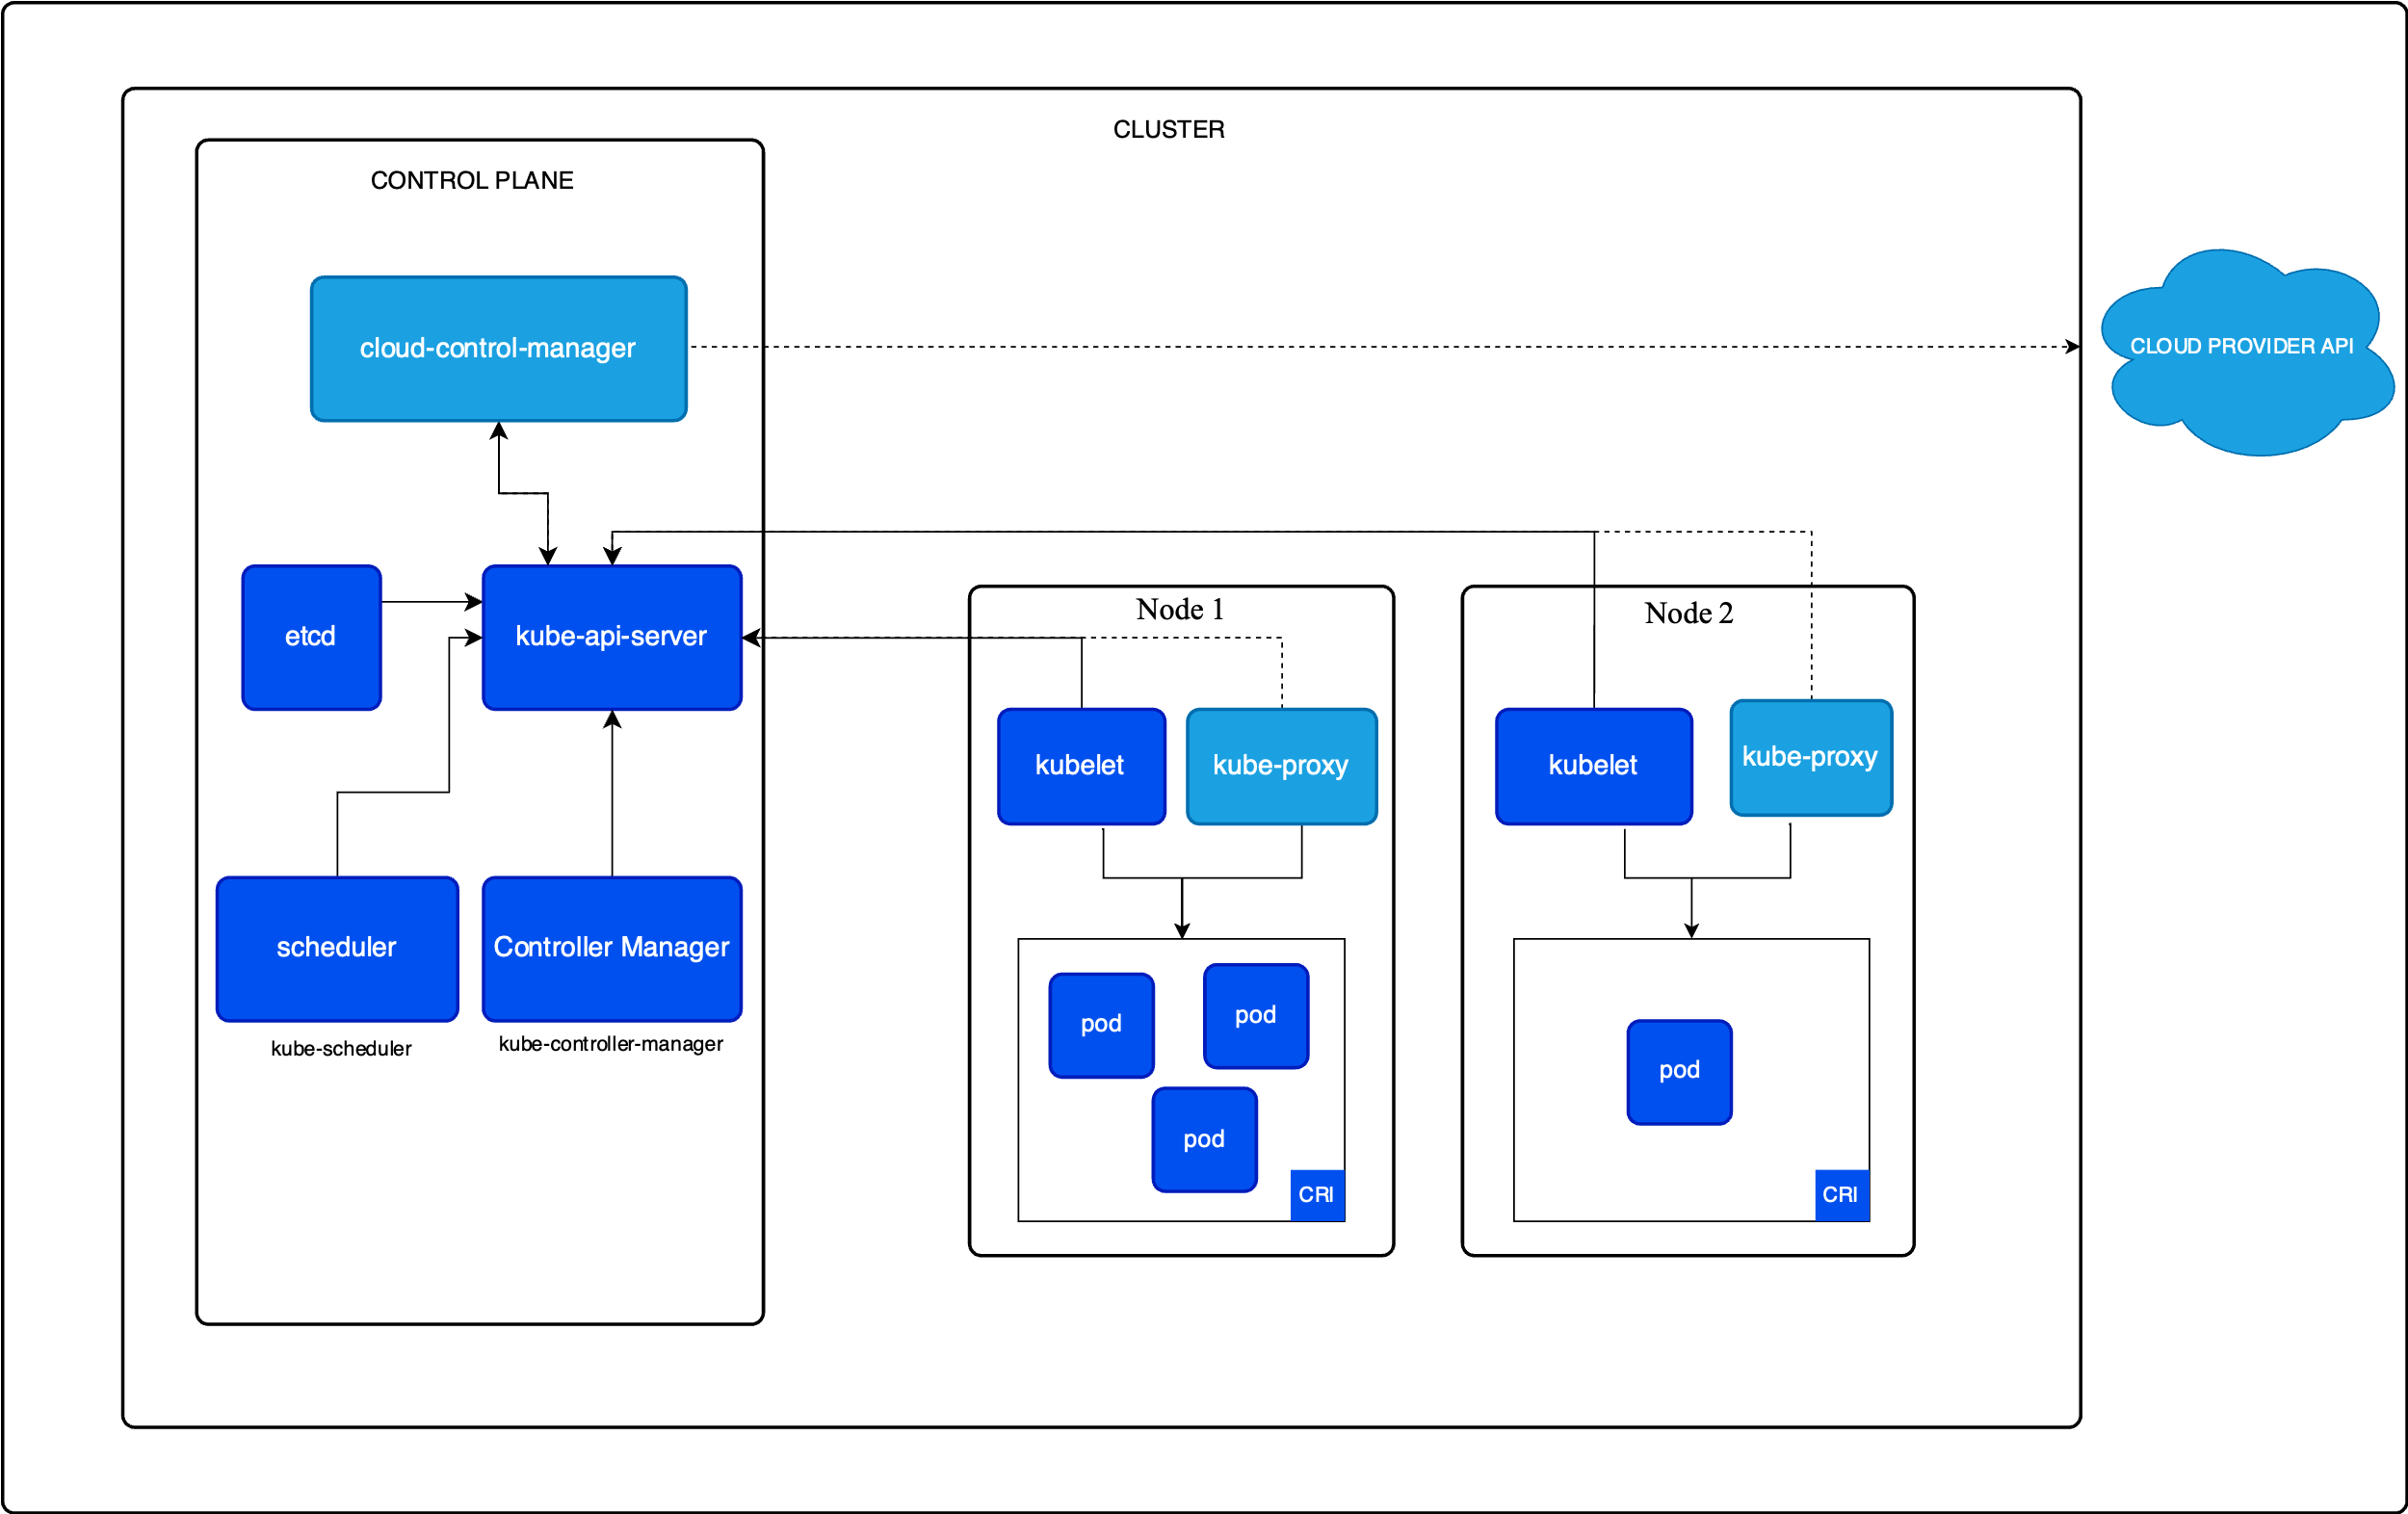
\includegraphics[keepaspectratio, width=0.8\textwidth]{src/resources/figures/image6.png}
    \caption{Arsitektur ElaX}
    \label{fig:elax-architecture}
\end{figure}

ElaX adalah kerangka kerja penskalaan yang bertujuan untuk mengoptimalkan penyediaan sumber daya bagi layanan cloud containerized, dengan tetap menjamin pemenuhan \emph{Service Level Objectives} (SLO) khususnya terkait dengan \emph{tail latency}. Dalam penelitian ini ElaX digunakan sebagai basis metode yang akan dimodifikasi. Terdiri dari 3 komponen utama, ditunjukkan pada Gambar~\ref{fig:elax-architecture}.

\begin{enumerate}
    \item \textbf{Prediktor Beban Kerja}
\end{enumerate}

Tersusun dari jaringan \emph{Long Short-Term Memory} (LSTM) untuk memprediksi beban kerja. Prediktor akan belajar dari data historis beban dan membuat prediksi pada beban kerja kedepan. Output prediksi beban kerja dari bagian ini akan masuk ke komponen reservasi sumber daya.

\begin{enumerate}
    \setcounter{enumi}{1}
    \item \textbf{Reservasi Sumber Daya}
\end{enumerate}

Merupakan model workload-resource yang berfungsi untuk mengestimasi kebutuhan sumberdaya berdasarkan hasil prediksi beban kerja. Terdiri dari model pemrograman matematis yang mempertimbangkan \emph{cost} ketika melakukan operasi \emph{scalling}. Kemudian model akan mengeluarkan keputusan untuk melakukan \emph{scale-up} dan \emph{scale-out} dengan cost paling sedikit.

\begin{enumerate}
    \setcounter{enumi}{2}
    \item \textbf{Pengendali Online}
\end{enumerate}

Kontroler bekerja berdasarkan nilai kondisi sekarang dibandingkan dengan SLO. Ketika \emph{tail latency} berada pada level kritis akan melanggar SLO, maka sumber daya akan disesuaikan, sebaliknya apabila telah berada pada level yang aman, maka reservasi sumber daya akan dilepas. Algoritma~\ref{alg:online-control} menunjukkan mekanisme pengendali online.

\begin{figure}[htbp]
\caption{Online Control Algorithm}
\label{alg:online-control}
\begin{algorithmic}[1]
\State \textbf{Variables:}
\State \quad $SLO\_target \gets \textbf{False}$
\State \quad $slack \gets 0$
\State \quad $cur\_resource$
\Repeat
    \State $slack \gets (SLO\_target - \text{GetTailLatency()}) / SLO\_target$
    \If{$slack > 0$}
        \State $\text{IncrResource}(cur\_resource \times 10\%)$
    \ElsIf{$0 < slack < 0.05$}
        \State $\text{IncrResource}(cur\_resource \times 5\%)$
    \Else
        \State $extra\_resource \gets cur\_resource - pre\_resource$
        \If{$extra\_resource > 0$}
            \State $\text{RemoveResource}(extra\_resource \times 50\%)$
        \EndIf
    \EndIf
    \State $\text{wait}(2)$ \Comment{Delay for 2 seconds}
\Until{forever}
\end{algorithmic}
\end{figure}
